\trilingualchapter{Opening Day: The Moment of Truth}{开业日:关键时刻}{Eröffnungstag: Der Moment der Wahrheit}{}

After months of planning, preparation, and anticipation, opening day arrives. This chapter follows Sue and Owen through their grand opening, covering final preparations, opening day execution, and the critical first weeks of operation.

\section{Final Preparations | 最终准备 | Letzte Vorbereitungen}

\begin{figure}[h]
\centering
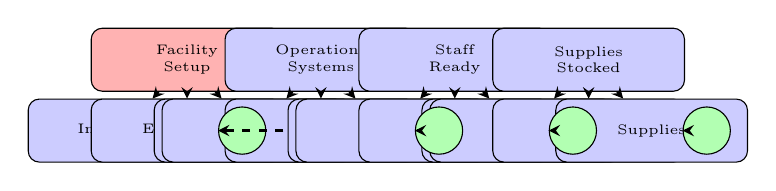
\begin{tikzpicture}[
    node distance=1.2cm,
    auto,
    prep/.style={rectangle, draw, fill=blue!20, text width=2.2cm, text centered, rounded corners, minimum height=0.8cm, font=\tiny},
    check/.style={circle, draw, fill=green!30, minimum size=0.6cm},
    arrow/.style={thick,->,>=stealth}
]
    % Preparation categories
    \node [prep, fill=red!30] (facility) {Facility\\Setup};
    \node [prep, right of=facility, xshift=0.5cm] (ops) {Operations\\Systems};
    \node [prep, right of=ops, xshift=0.5cm] (staff) {Staff\\Ready};
    \node [prep, right of=staff, xshift=0.5cm] (supplies) {Supplies\\Stocked};
    
    % Sub-items
    \node [prep, below of=facility, yshift=0.3cm, xshift=-0.8cm] (f1) {Inspections};
    \node [prep, below of=facility, yshift=0.3cm] (f2) {Equipment};
    \node [prep, below of=facility, yshift=0.3cm, xshift=0.8cm] (f3) {Cleaning};
    
    \node [prep, below of=ops, yshift=0.3cm, xshift=-0.8cm] (o1) {Licenses};
    \node [prep, below of=ops, yshift=0.3cm] (o2) {POS};
    \node [prep, below of=ops, yshift=0.3cm, xshift=0.8cm] (o3) {Tech};
    
    \node [prep, below of=staff, yshift=0.3cm, xshift=-0.8cm] (s1) {Hired};
    \node [prep, below of=staff, yshift=0.3cm] (s2) {Trained};
    \node [prep, below of=staff, yshift=0.3cm, xshift=0.8cm] (s3) {Scheduled};
    
    \node [prep, below of=supplies, yshift=0.3cm, xshift=-0.8cm] (su1) {Food};
    \node [prep, below of=supplies, yshift=0.3cm] (su2) {Beverage};
    \node [prep, below of=supplies, yshift=0.3cm, xshift=0.8cm] (su3) {Supplies};
    
    % Check marks
    \node [check, right of=f1, xshift=0.3cm] (c1) {};
    \node [check, right of=o2, xshift=0.3cm] (c2) {};
    \node [check, right of=s2, xshift=0.3cm] (c3) {};
    \node [check, right of=su2, xshift=0.3cm] (c4) {};
    
    % Arrows
    \draw [arrow] (facility) -- (f1);
    \draw [arrow] (facility) -- (f2);
    \draw [arrow] (facility) -- (f3);
    \draw [arrow] (ops) -- (o1);
    \draw [arrow] (ops) -- (o2);
    \draw [arrow] (ops) -- (o3);
    \draw [arrow] (staff) -- (s1);
    \draw [arrow] (staff) -- (s2);
    \draw [arrow] (staff) -- (s3);
    \draw [arrow] (supplies) -- (su1);
    \draw [arrow] (supplies) -- (su2);
    \draw [arrow] (supplies) -- (su3);
    
    % Check connections
    \draw [arrow, dashed] (f2) -- (c1);
    \draw [arrow, dashed] (o2) -- (c2);
    \draw [arrow, dashed] (s2) -- (c3);
    \draw [arrow, dashed] (su2) -- (c4);
\end{tikzpicture}
\caption{Pre-Opening Preparation Checklist}
\label{fig:prep_checklist}
\end{figure}

\subsection{Pre-Opening Checklist}

In the weeks leading up to opening, Sue and Owen completed a comprehensive checklist:

\subsubsection{Facility}
\begin{itemize}
    \item Final inspections (health, fire, building)
    \item All equipment tested and operational
    \item Utilities confirmed (gas, electric, water)
    \item Cleaning and deep cleaning completed
    \item Signage installed and lit
    \item Parking and accessibility verified
\end{itemize}

\subsubsection{Operations}
\begin{itemize}
    \item All licenses and permits obtained
    \item Insurance policies active
    \item POS system tested and trained
    \item Reservation system operational
    \item Phone system working
    \item Wi-Fi and technology functional
\end{itemize}

\subsubsection{Staff}
\begin{itemize}
    \item All positions filled
    \item Training completed
    \item Uniforms and equipment distributed
    \item Schedules posted
    \item Emergency contacts available
\end{itemize}

\subsubsection{Supplies}
\begin{itemize}
    \item Initial inventory received and stored
    \item All smallwares and supplies stocked
    \item Cleaning supplies available
    \item Office supplies ready
\end{itemize}

\subsection{Soft Opening | 试营业 | Soft Opening}

Before the public opening, Sue and Owen held a soft opening:

\subsubsection{Purpose}
\begin{itemize}
    \item Test all systems and procedures
    \item Train staff in real conditions
    \item Identify and fix issues
    \item Build confidence
    \item Generate initial buzz
\end{itemize}

\subsubsection{Invitees}
\begin{itemize}
    \item Friends and family
    \item Industry contacts
    \item Local media and influencers
    \item Neighbors and community leaders
    \item Staff families
\end{itemize}

\subsubsection{What to Test}
\begin{itemize}
    \item Kitchen timing and flow
    \item Service procedures
    \item POS system functionality
    \item Reservation management
    \item Food quality and consistency
    \item Table turnover
    \item Communication between FOH and BOH
\end{itemize}

\section{Opening Day Strategy | 开业日策略 | Eröffnungstag-Strategie}

\subsection{Managing Expectations | 管理期望 | Erwartungen managen}

Sue and Owen set realistic expectations:
\begin{itemize}
    \item Expect some issues (normal for opening)
    \item Focus on hospitality over perfection
    \item Have extra staff for support
    \item Prepare for higher than normal volume
    \item Be present and visible
\end{itemize}

\subsection{Staffing for Opening | 开业人员配置 | Personal für die Eröffnung}

\begin{itemize}
    \item Overstaff slightly for support
    \item Have managers on all shifts
    \item Extra support staff (bussers, runners)
    \item Backup staff on call
    \item Clear roles and responsibilities
\end{itemize}

\subsection{Menu Strategy | 菜单策略 | Menüstrategie}

\begin{itemize}
    \item Start with core menu items
    \item Limit complexity initially
    \item Ensure all items are well-tested
    \item Have backup options ready
    \item Be prepared to 86 items if needed
\end{itemize}

\section{Opening Day Execution | 开业日执行 | Eröffnungstag-Durchführung}

\subsection{Morning Preparation | 早晨准备 | Morgenvorbereitung}

\begin{itemize}
    \item Early arrival (2-3 hours before service)
    \item Final walkthrough
    \item Staff briefing
    \item Equipment checks
    \item Inventory verification
    \item Mise en place completion
    \item Final cleaning touches
\end{itemize}

\subsection{During Service | 服务期间 | Während des Service}

\subsubsection{Management Presence}
\begin{itemize}
    \item Sue in kitchen, monitoring food quality
    \item Owen on floor, managing service
    \item Both available for problem-solving
    \item Regular communication
\end{itemize}

\subsubsection{Key Priorities}
\begin{itemize}
    \item Guest satisfaction above all
    \item Food quality and safety
    \item Service standards
    \item Problem resolution
    \item Team support
\end{itemize}

\subsubsection{Common Issues and Solutions}
\begin{itemize}
    \item \textbf{Kitchen delays}: Communicate with guests, offer drinks
    \item \textbf{Service mistakes}: Apologize, fix immediately, comp if appropriate
    \item \textbf{Equipment issues}: Have backup plans
    \item \textbf{Staff confusion}: Clear communication, support
    \item \textbf{Overwhelming volume}: Manage reservations, communicate waits
\end{itemize}

\subsection{End of Day | 一天结束 | Tagesende}

\begin{itemize}
    \item Thank staff
    \item Quick debrief
    \item Note issues for follow-up
    \item Clean and reset for next day
    \item Rest and prepare for tomorrow
\end{itemize}

\section{First Week | 第一周 | Erste Woche}

\subsection{Daily Routine | 日常例行 | Tägliche Routine}

\begin{itemize}
    \item Morning briefing with staff
    \item Review previous day's performance
    \item Address issues immediately
    \item Adjust as needed
    \item Evening debrief
    \item Plan for next day
\end{itemize}

\subsection{Key Focus Areas | 关键关注领域 | Wichtige Fokusbereiche}

\subsubsection{Operations}
\begin{itemize}
    \item Refine timing and flow
    \item Adjust staffing levels
    \item Fix equipment issues
    \item Improve communication
    \item Standardize procedures
\end{itemize}

\subsubsection{Quality}
\begin{itemize}
    \item Maintain food quality
    \item Ensure service standards
    \item Address customer feedback
    \item Train and retrain as needed
\end{itemize}

\subsubsection{Team}
\begin{itemize}
    \item Support staff through learning curve
    \item Recognize good performance
    \item Address concerns promptly
    \item Build team cohesion
\end{itemize}

\section{Managing Challenges | 管理挑战 | Herausforderungen bewältigen}

\subsection{Common Opening Challenges | 常见开业挑战 | Häufige Eröffnungsh Herausforderungen}

\subsubsection{Operational}
\begin{itemize}
    \item Equipment malfunctions
    \item Supply shortages
    \item Staff turnover
    \item Inconsistent execution
    \item System glitches
\end{itemize}

\subsubsection{Customer}
\begin{itemize}
    \item Long wait times
    \item Service issues
    \item Quality concerns
    \item Unrealistic expectations
    \item Negative reviews
\end{itemize}

\subsection{Problem-Solving Approach | 问题解决方法 | Problemlösungsansatz}

\begin{enumerate}
    \item Acknowledge the issue
    \item Assess impact and urgency
    \item Develop solution
    \item Implement quickly
    \item Monitor results
    \item Adjust if needed
    \item Learn for future
\end{enumerate}

\section{Customer Feedback | 客户反馈 | Kundenfeedback}

\subsection{Collecting Feedback | 收集反馈 | Feedback sammeln}

\begin{itemize}
    \item Table visits during service
    \item Comment cards
    \item Online reviews
    \item Social media monitoring
    \item Staff observations
\end{itemize}

\subsection{Responding to Feedback | 回应反馈 | Auf Feedback reagieren}

\begin{itemize}
    \item Thank customers for feedback
    \item Address concerns immediately
    \item Follow up when appropriate
    \item Use feedback for improvement
    \item Share positive feedback with team
\end{itemize}

\section{Marketing During Opening | 开业期间的营销 | Marketing während der Eröffnung}

\subsection{Grand Opening Events | 盛大开业活动 | Große Eröffnungsveranstaltungen}

\begin{itemize}
    \item Ribbon cutting ceremony
    \item Media coverage
    \item Social media posts
    \item Special promotions
    \item Community engagement
\end{itemize}

\subsection{Generating Buzz | 制造话题 | Aufmerksamkeit erzeugen}

\begin{itemize}
    \item Encourage social media check-ins
    \item Share behind-the-scenes content
    \item Respond to all reviews
    \item Engage with local community
    \item Partner with influencers
\end{itemize}

\section{Financial Monitoring | 财务监控 | Finanzüberwachung}

\subsection{Daily Tracking | 日常跟踪 | Tägliche Verfolgung}

\begin{itemize}
    \item Sales volume
    \item Food and labor costs
    \item Customer counts
    \item Average check
    \item Cash flow
\end{itemize}

\subsection{Adjustments | 调整 | Anpassungen}

\begin{itemize}
    \item Pricing if needed
    \item Portion sizes
    \item Staffing levels
    \item Menu items
    \item Operating hours
\end{itemize}

\trilingualsection{Key Takeaways}{关键要点}{Wichtige Erkenntnisse}{}

\begin{itemize}
    \item Preparation is critical—complete checklists thoroughly
    \item Soft opening is invaluable for testing
    \item Expect issues and be ready to solve them
    \item Overstaff initially for support
    \item Focus on hospitality and guest satisfaction
    \item Be present and visible on opening day
    \item Address problems immediately
    \item Collect and act on feedback
    \item Monitor financials daily
    \item Adjust quickly based on reality
\end{itemize}

Opening day marked the beginning of Sue and Owen's restaurant journey. While challenging, it was also exhilarating. With the opening behind them, they now faced the ongoing challenge of building a sustainable, successful operation. The next chapter explores the day-to-day operations and long-term sustainability of a restaurant.
